\documentclass[12pt]{extarticle}
\usepackage[utf8]{inputenc}
\usepackage{graphicx}
\usepackage{float}

% Disable indentation
\setlength{\parindent}{0pt}

\title{Lab 7: Network virtualization with Virtualbox}
\author{Alexander Hoffmann}
\date{\today}

\begin{document}

\maketitle

\section{NAT mode}
\textbf{1.} The IP configuration of the host machine can be determined using \texttt{ifconfig}.\\~\\
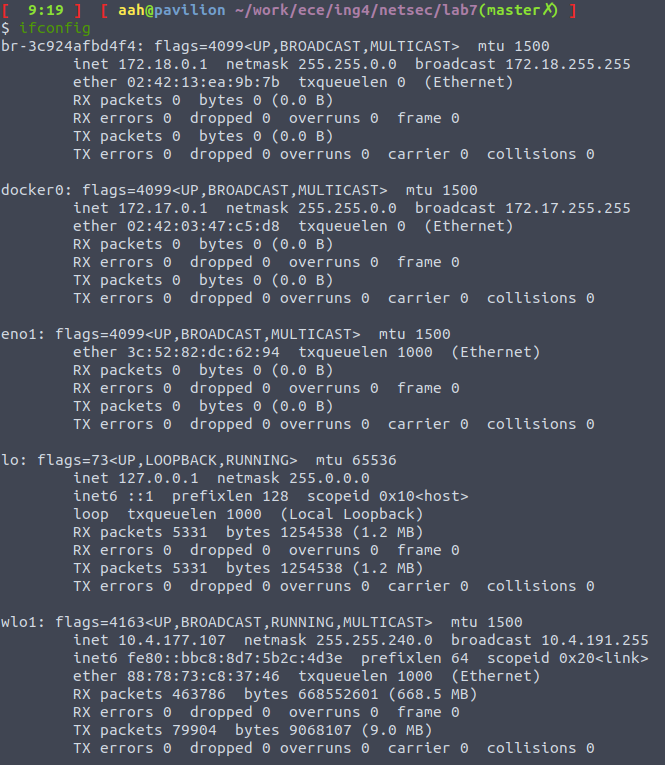
\includegraphics[scale=0.6]{resources/1-1.png}\\

\textbf{2.} We use the same command in the virtual machine.\\~\\
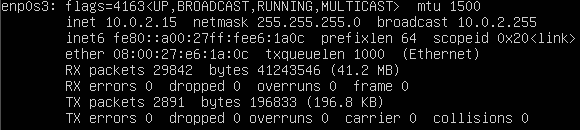
\includegraphics[scale=0.7]{resources/1-2.png}\\

\textbf{3.} It seems like the host machine and the virtual machine are not on the same network. This is because the VM is connected through NAT.\\

\textbf{4.} To get the DHCP server address, we use the following command:
\begin{verbatim}
sudo grep -R "DHCPOFFER" /var/log/*
\end{verbatim}
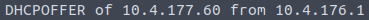
\includegraphics[scale=0.7]{resources/1-4.png}\\
This corresponds to the DHCP server address on the host machine. Now let's see which IP the DHCP server has on the VM.\\~\\
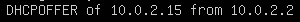
\includegraphics[scale=0.8]{resources/1-4-2.png}\\

\textbf{5.} The IP address of the NAT device is 10.0.2.15.

\textbf{6.} Since the VM is a server, it does not have a virtual interface. Therefore, we will be using \texttt{tcpdump} to capture traffic. More specifically, to filter the DHCP protocol, we use the following:
\begin{verbatim}
tcpdump -i eth0 -pvn port 67 and port 68
\end{verbatim}
Now we have to renew the DHCP lease. To do this, use:
\begin{verbatim}
dhclient enp0s3
\end{verbatim}
Which will display the following packets.\\~\\
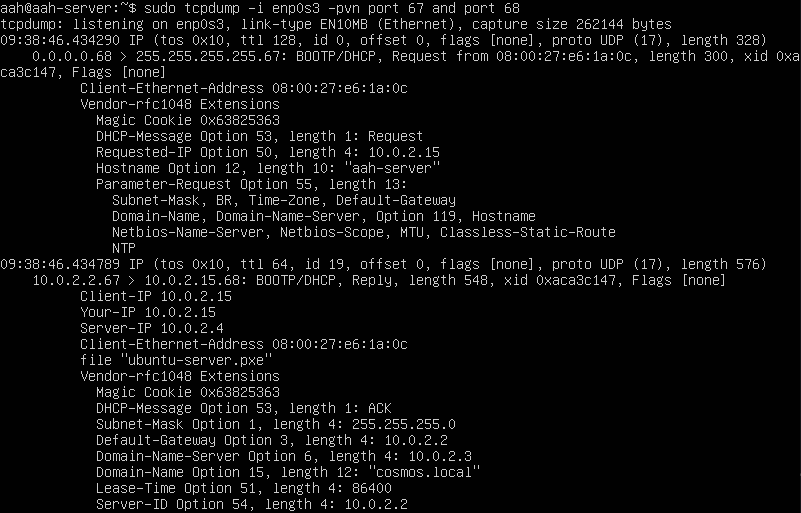
\includegraphics[scale=0.5]{resources/1-5.png}\\
We can observe that the VM broadcasts a DHCP Request. The DHCP server then sends a DHCP Reply with a lease.

\textbf{7.} There is no direct traffic between the DHCP server and the VM. In fact, the host machine is the DHCP server for the VM. This is why we are not capturing any traffic going to the VM.\\~\\
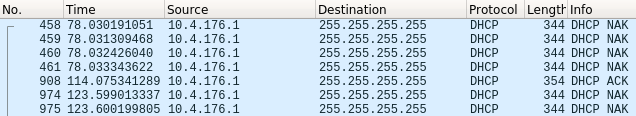
\includegraphics[scale=0.6]{resources/1-7.png}\\

\textbf{8.} Once again, since the VM does not have a graphical interface, we will use the \texttt{ping} command to observe the traffic. Suppose we ping google.com from the VM. Here is the traffic captured by Wireshark on the host machine.\\~\\
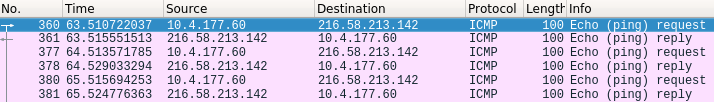
\includegraphics[scale=0.6]{resources/1-8.png}\\
Now let's observe the ping from the host.\\~\\
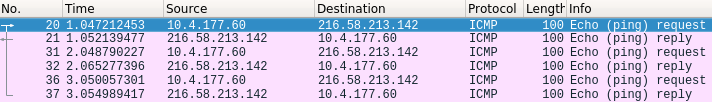
\includegraphics[scale=0.6]{resources/1-8-1.png}\\
The packets are simingly the same except that the header is slightly different.

\end{document}
